\section{Replacing single statements with block statements}

Given the fact that Java allows some statements to appear outside of a block, they may cause problems in later steps of
the algorithm when processing the statements of a block. For example, if a new statement needs to be added before or
after another statement which is not part of a block, the initial statement needs to be first enclosed in a block, in
which the other statement will be added at the right place.
The places where this pass is applied are the branches of
\code{if}\footnote{\url{https://docs.oracle.com/javase/specs/jls/se8/html/jls-14.html#jls-14.9}} statements and the
bodies of \code{for}\footnote{\url{https://docs.oracle.com/javase/specs/jls/se8/html/jls-14.html#jls-14.14.1}},
\code{foreach}\footnote{\url{https://docs.oracle.com/javase/specs/jls/se8/html/jls-14.html#jls-14.14.2}},
\code{while}\footnote{\url{https://docs.oracle.com/javase/specs/jls/se8/html/jls-14.html#jls-14.12}} and
\code{do-while}\footnote{\url{https://docs.oracle.com/javase/specs/jls/se8/html/jls-14.html#jls-14.13}} statements
which contain single statements. If the single statement is an instance of
\code{PsiEmptyStatement}\footnote{\url{https://docs.oracle.com/javase/specs/jls/se8/html/jls-14.html#jls-14.6}},
it gets replaced with an empty block instead of a block containing an empty statement, because this would be redundant.

A special case is the \code{switch}\footnote{\url{https://docs.oracle.com/javase/specs/jls/se8/html/jls-14.html#jls-14.11}}
statement. The pass replaces the statements after each \code{switch} label (both \code{case} and \code{default} labels)
up to the next \code{switch} label (no next one when the label is the last) with a block containing these statements.
This transformation does not alter the semantics of the \code{switch} statement.

This pass also transforms statements which may not contain recursive calls, because there are elements which the
refactoring alters in order to remove recursion and they are not only method calls (for example, \code{return}
statements). An example is provided in \labelindexref{Figure}{img:replace-single-statements-with-block-statements}.

\begin{figure}[htb]
    \makebox[\linewidth][c]{%
    \begin{subfigure}[b]{.6\textwidth}
        \centering
        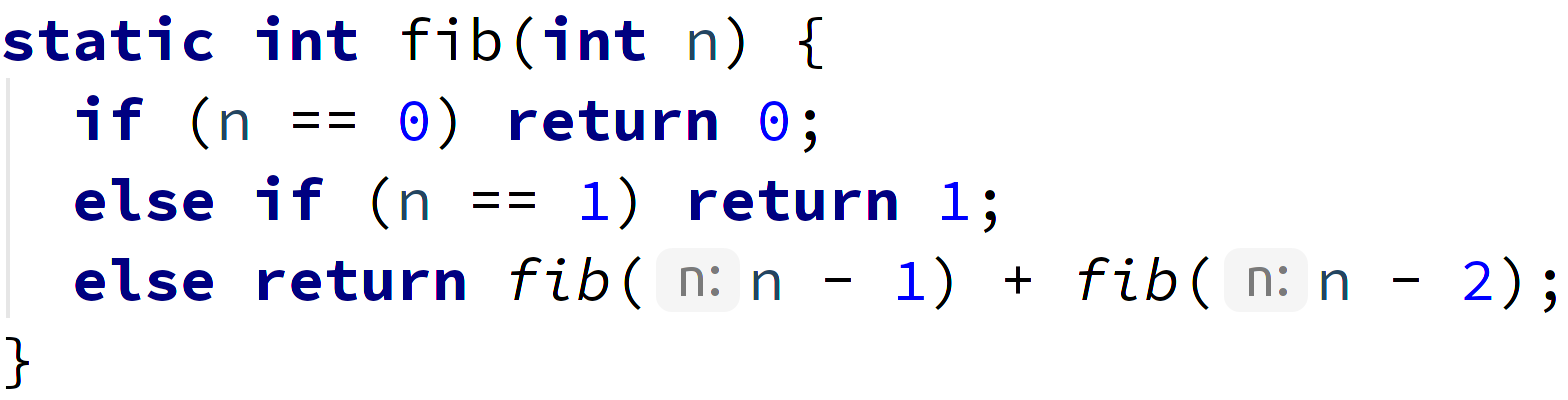
\includegraphics[height=0.6in]{src/img/replace-single-statements-with-block-statements-before-white.png}
        \caption{Before}
    \end{subfigure}%
    \begin{subfigure}[b]{.6\textwidth}
        \centering
        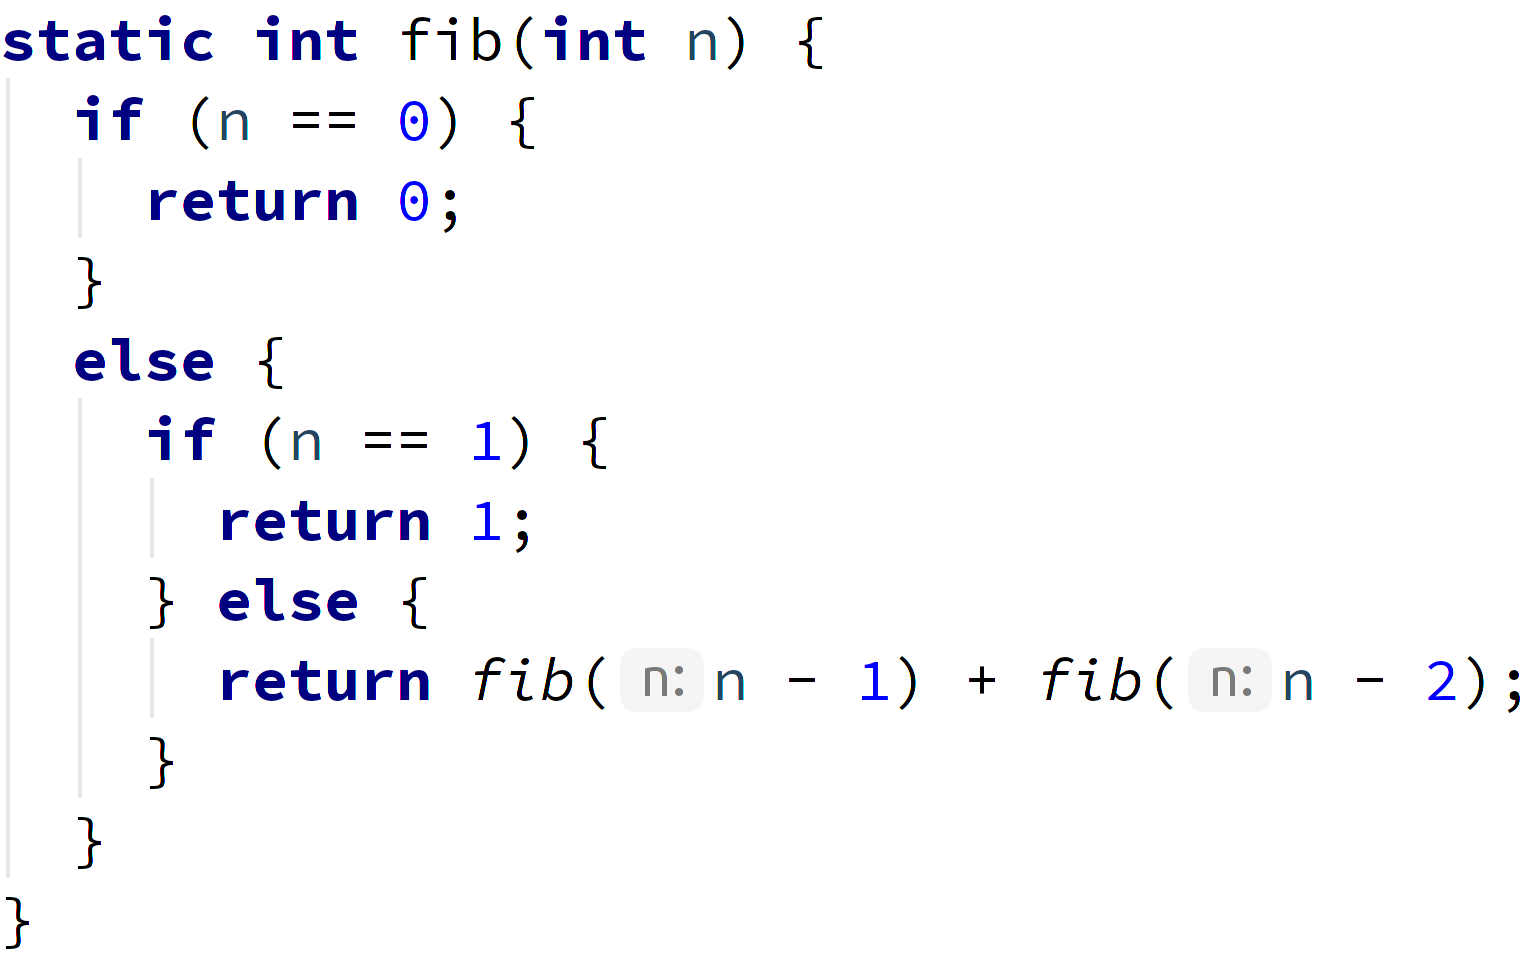
\includegraphics[height=1.44in]{src/img/replace-single-statements-with-block-statements-after-white.png}
        \caption{After}
    \end{subfigure}%
    }\\
    \caption{Replacing single statements with block statements \label{img:replace-single-statements-with-block-statements}}
\end{figure}